\chapter{Results} \label{chap:res}

\section{Analysis of Olympic Games Duration and Evolution}

The Gantt chart in Figure \ref{fig:gantt_olympics} illustrates the scheduling and duration of both Summer and Winter Olympic Games from the inaugural Athens Games in 1896 to the events in 2022. It highlights key milestones and trends in the evolution of the Olympics.

\begin{figure}[ht]
    \centering
    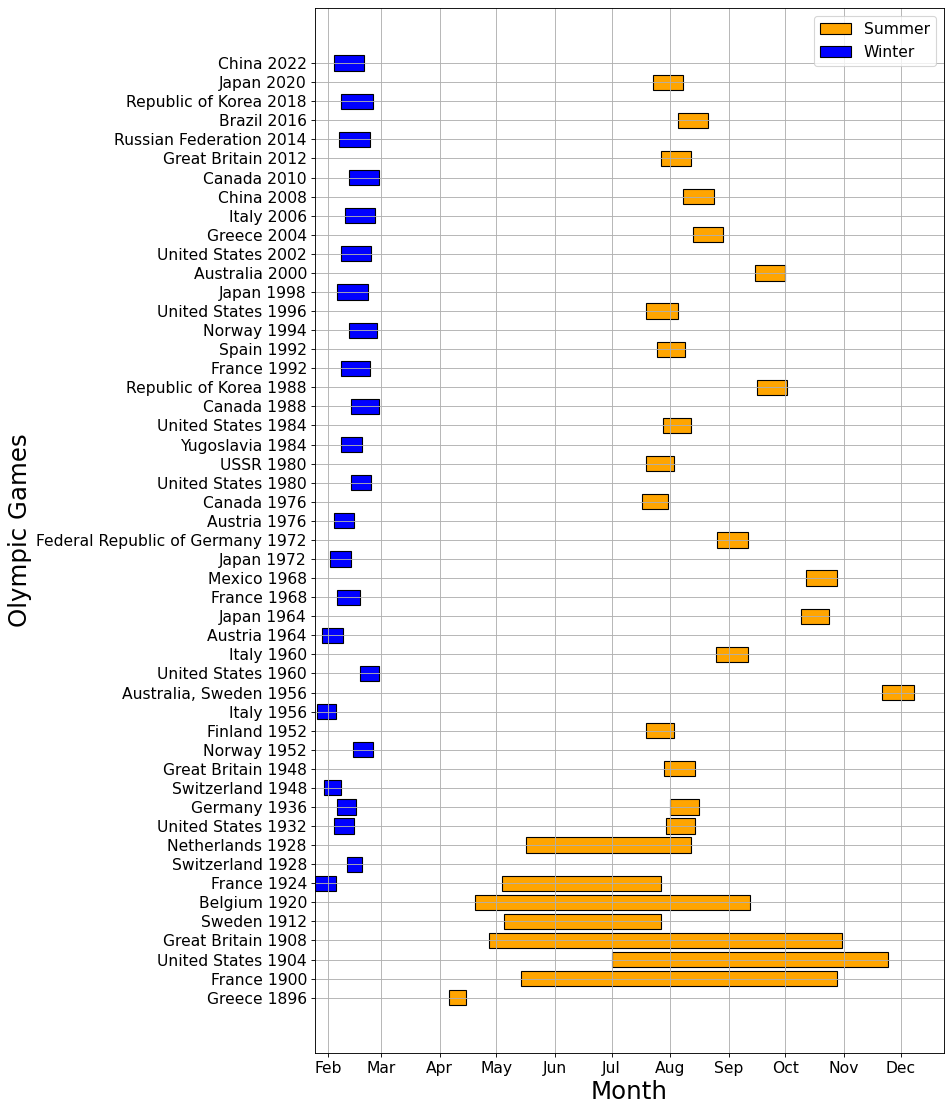
\includegraphics[width=0.8\textwidth]{Gantt Chart of Olympic Games.png}
    \caption{Gantt Chart of Olympic Games Duration}
    \label{fig:gantt_olympics}
\end{figure}

The modern Olympics began in 1896 with exclusively male participants and a limited schedule of events lasting 10 days. By 1900, the Paris Games introduced women's participation and expanded the schedule to over five months, integrating the Olympics into the World’s Fair. This unusual duration reflected the scattered organization and the addition of new sports like golf, tennis, and rowing. Over time, the duration became more standardized, with events typically lasting around two weeks by the mid-20th century, reflecting the Games' growing scale and complexity.

The Winter Olympics were introduced in Chamonix, France, in 1924, marking the start of a separate seasonal competition for winter sports. Notably, France hosted both the Summer and Winter Games in the same year, solidifying its pivotal role in Olympic history.

Additionally, the chart captures regular scheduling patterns, with Summer Games typically held between July and August and Winter Games in February. It also reveals disruptions caused by global conflicts, including cancellations during World War I and World War II.

\section{Chord Diagram for Migration Flow}

PLACEHOLDER ...

\section{Dynamic Choropleths and Bubble Maps}

The dynamic choropleth and bubble maps were designed to provide an interactive exploration of Olympic trends worldwide. These maps enable users to visualize data such as the frequency of Olympic hosting by country, the number of athlete debuts, and medal counts. With dynamic filtering options and multiple visualization styles, they offer a versatile and engaging way to analyze key aspects of Olympic history.

The choropleth map excels at conveying spatial patterns and regional comparisons through color intensity, making it ideal for quickly identifying geographical trends. However, it may obscure information for smaller countries due to their limited map space. In contrast, the bubble map highlights individual data points with proportional circle sizes, ensuring that smaller countries remain visible and providing a more precise representation of numerical values. On the downside, bubble maps can become cluttered in regions with dense data points, potentially making it harder to interpret overlapping bubbles. Together, these visualization styles complement each other, balancing clarity and detail depending on the user's analytical needs.

\begin{figure}[ht]
    \centering
    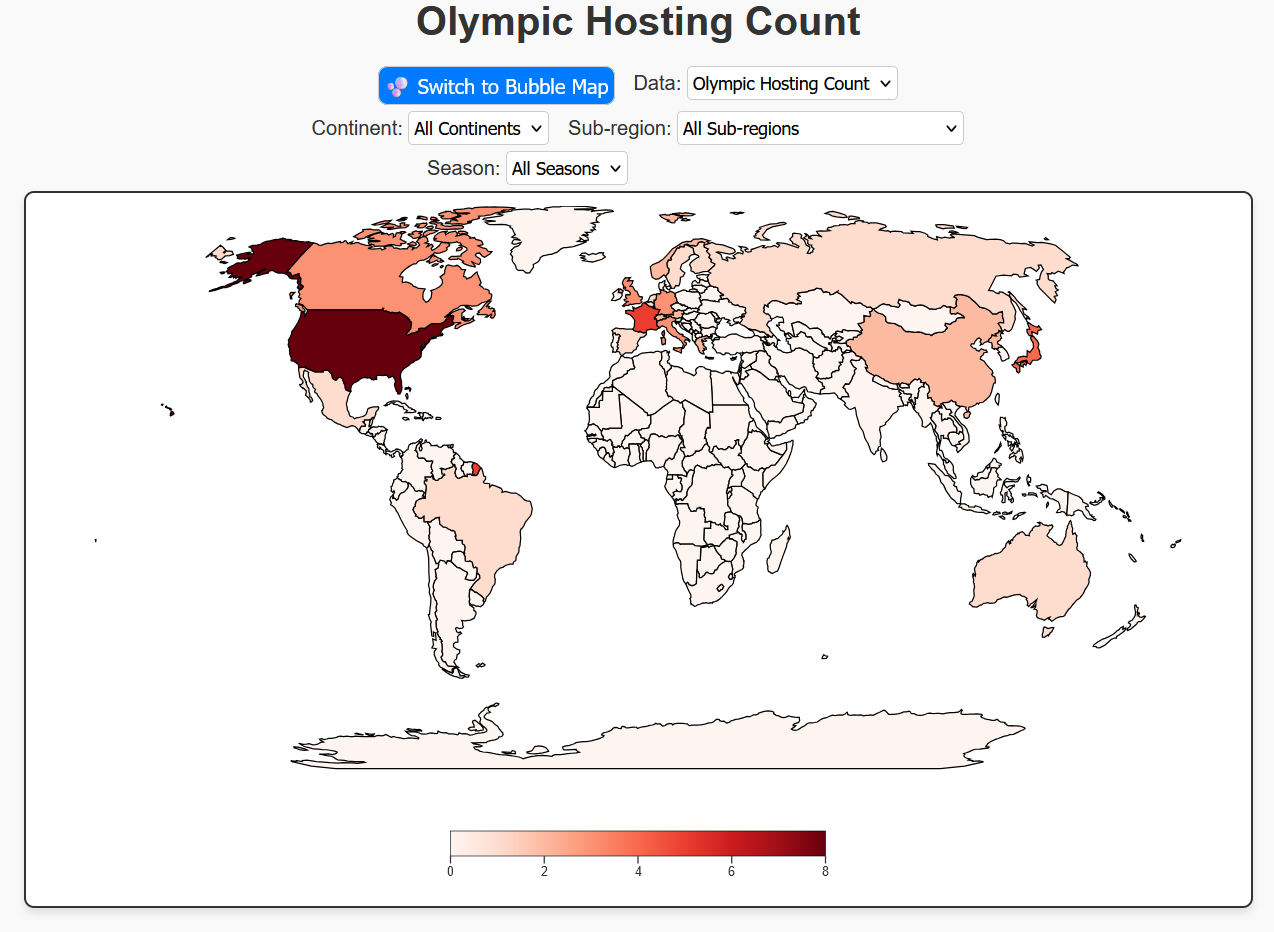
\includegraphics[width=0.8\textwidth]{Dynamic Choropleth.png}
    \caption{Dynamic Choropleth Map: Visualizing Olympic Hosting Trends}
    \label{fig:choropleth_map}
\end{figure}

\begin{figure}[ht]
    \centering
    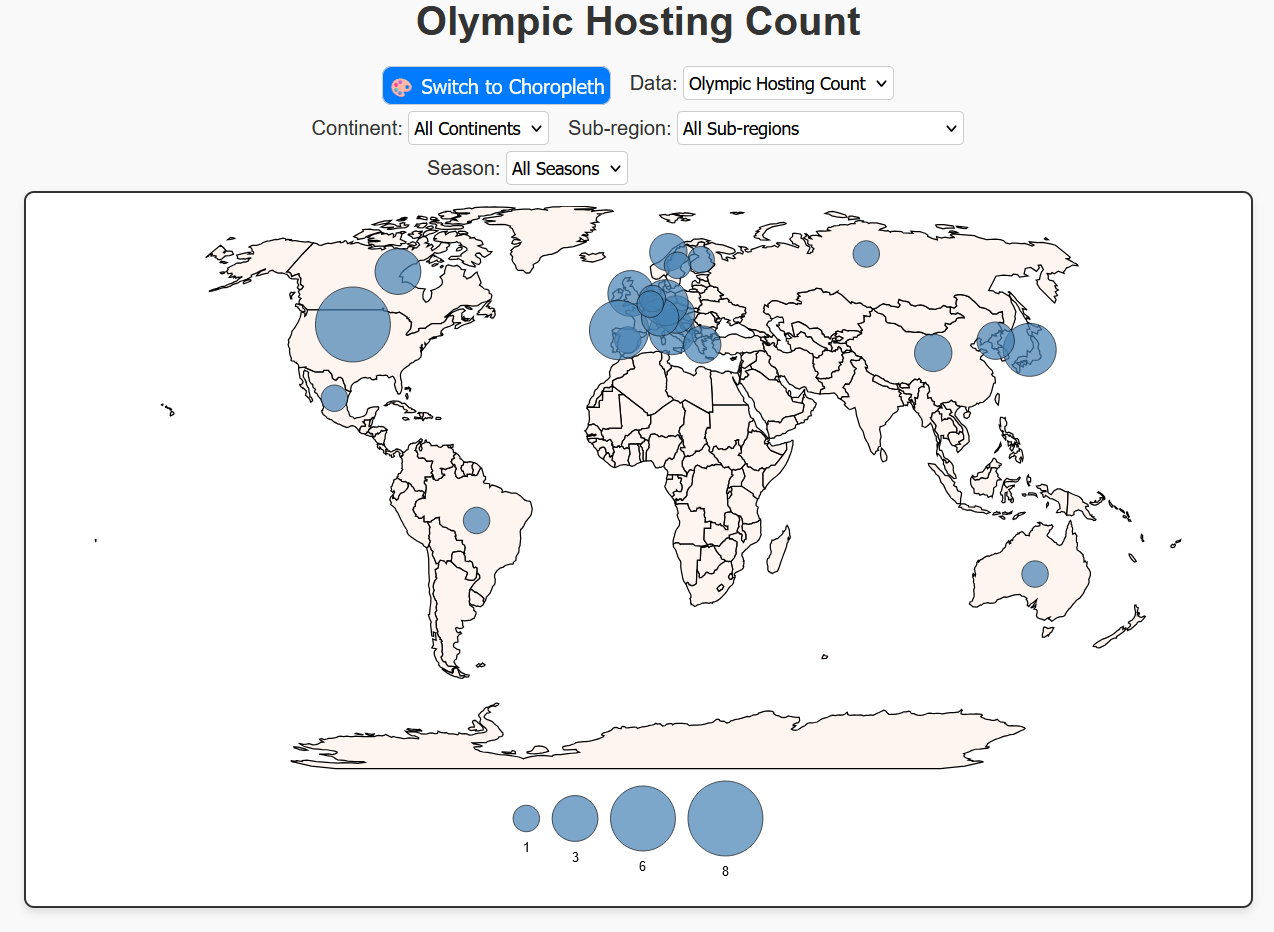
\includegraphics[width=0.8\textwidth]{Dynamic Bubble Map.png}
    \caption{Dynamic Bubble Map: Visualizing Olympic Hosting Trends}
    \label{fig:bubble_map}
\end{figure}

\subsection{Features of the Maps}

The maps provide the following functionalities:
\begin{itemize}
    \item \textbf{Visualization Modes:} Users can switch between a choropleth map (Figure \ref{fig:choropleth_map}) and a bubble map (Figure \ref{fig:bubble_map}) for different visual representations of hosting frequency.
    \item \textbf{Filters and Options:} Filtering options include continents, sub-regions, seasons (Summer or Winter), medal types (Gold, Silver or Bronze), if applicable. These allow users to customize the view and focus on specific geographic or temporal trends.
    \item \textbf{Interactivity:} Both maps feature hover-over tooltips displaying detailed information, such as the number of times a country has hosted the Olympics.
\end{itemize}

\subsection{Insights from the Maps}

These maps reveal several insights into Olympic hosting trends:
\begin{itemize}
    \item Countries such as the United States, Great Britain, and France stand out in number of debuts and high hosting frequencies, reflecting their longstanding involvement in the Olympics.
    \item Hosting occurrences are concentrated in Europe and North America, particularly during the early years of the modern Olympics.
    \item The inclusion of filtering options enables the identification of hosting trends by region, season, and medal type, highlighting the geographical expansion of the Games over time.
\end{itemize}

The combination of choropleth and bubble maps exemplifies the power of interactive visualizations, enabling a flexible exploration of the data while revealing key trends and disparities in Olympic hosting.

\section{ADNANE PLOTS}

PLACEHOLDER
